\documentclass[number=03]{assignment}
\title{Computer Architecture - TE2031}
\chead{Second Partial Project 2/3}
\rhead{I-Type}
%\date{February - June 2020}

\newif\ifanswers
\answerstrue % comment out to hide answers

% TOP
\newcommand{\mipspkgfile}{\colorfilename{mips\_pkg.sv}}
\newcommand{\rtypefile}{\colorfilename{rtype.sv}}
\newcommand{\rtypetbfile}{\colorfilename{tb\_rtype.sv}}
\newcommand{\rtypedofile}{\colorfilename{rtype.do}}

\newcommand{\itypefile}{\colorfilename{itype.sv}}
\newcommand{\itypetbfile}{\colorfilename{tb\_itype.sv}}
\newcommand{\itypedofile}{\colorfilename{itype.do}}

% MUX
\newcommand{\muxfile}[1]{\colorfilename{mux\_#1x1.sv}}
%\newcommand{\mux2x1file}[1]{\code{mux\_2x1.sv}}
\newcommand{\muxpkgfile}{\colorfilename{mux\_pkg.sv}}

% RF
\newcommand{\rfpkgfile}{\colorfilename{rf\_pkg.sv}}
\newcommand{\rffile}{\colorfilename{rf.sv}}
\newcommand{\tbrffile}{\colorfilename{tb\_rf.sv}}
\newcommand{\dorffile}{\colorfilename{rf.do}}

% ALU
\newcommand{\alupkgfile}{\colorfilename{alu\_pkg.sv}}
\newcommand{\alufile}{\colorfilename{alu.sv}}
\newcommand{\tbalufile}{\colorfilename{tb\_alu.sv}}

% SIGN EXTENDER
\newcommand{\sgnextfile}{\colorfilename{sgn\_ext.sv}}
\newcommand{\tbsgnextfile}{\colorfilename{tb\_sgn\_ext.sv}}

% CONTROL UNIT
\newcommand{\controlfile}{\colorfilename{control\_unit.sv}}

% DATA MEMORY
\newcommand{\dmfile}{\colorfilename{dm.sv}}

% GRADE WEIGHT
\newcommand{\DeliveryWeight}{This delivery constitutes 60\% of your second partial final grade.}

% DEADLINE
\newcommand{\deadline}{23:59 hours on Wednesday October 21st 2020}

\makesavenoteenv{tabular}
\makesavenoteenv{table}
% Begin document
\begin{document}

\setcounter{chapter}{1}
\chapter*{Second Partial Project \\ Delivery 2/3 \\ MIPS I-Type datapath}
% ======================================
% Objective
% ======================================
\section{Objectives}
To implement the datapath of a custom \ac{MIPS} \Itype instruction in \SV.  

% ======================================
% Second Partial weight
% ======================================
\section{Second partial grade weight}
\alertblue{\DeliveryWeight}
% ======================================
% Deadline
% ======================================
\section{Deadline}
\alertblue{\deadline}

% ======================================
% Teamwork policy
% ======================================
%\section{Teamwork policy}
%This is a group assignment. 
% ======================================
% Pre-requisites
% ======================================
\section{Pre-requisites}
It is assumed that you are familiar with working with \ModelSim and \Quartus. 
If you require assistance, you can refer to the first assignment tutorial.
It is assumed that you have completed the previous assignment for modelling the \ac{MIPS} \Rtype instructions in \SV.

%\acresetall
\newpage
% ======================================
% Background
% ======================================
\section{Background}
\fref{Figure:MIPS_IType_encoding} shows the encoding used in \Itype instructions.
%
\begin{figure}[!htb]
\centering
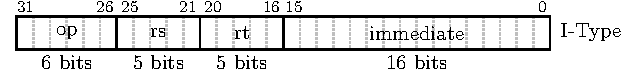
\includegraphics[scale=1.3]{MIPS_IType}
\caption{\ac{MIPS} \Itype instruction encoding.}
\label{Figure:MIPS_IType_encoding}
\end{figure}
%

As shown in, \fref{Figure:MIPS_IType_encoding}, an immediate value is specified directly in the lower half of the \Itype instruction encoding. 
This immediate value is then used: 1) as an operand in arithmetic or logical operations; 2) as an offset address for load/store instructions using displacement addressing modes; or 3) as the branch address in branch instructions. 
Field \code{op} of \fref{Figure:MIPS_IType_encoding} specifies the instruction to perform, whilst \code{rs} and \code{rt} are used as source and destination registers, respectively.


% ======================================
% Specifications
% ======================================
\section{Design specifications}
The following sections provide an overview of the design specifications for this assignment.

\subsection{General specifications}\label{sec:general_specs}
Your custom \ac{MIPS} design must comply with the following design specifications.
%
\begin{itemize}
\item Instruction set based (but modified) on a standard 16-bit \ac{MIPS} \ac{uP}.
\item Single-cycle design.
\item Data width is 16-bits.
\item Instruction encoding (instruction width) is 32-bits long.
\item \ac{RF} contains 32 registers.
\begin{itemize}
\item \code{r0} \alertblue{must} always be 0, \ie, \code{r0} is not writeable.
\item \code{r31} is return address.
\end{itemize}
\item \ac{IM} is parameterizable.
\item \ac{DM} is parameterizable.
\end{itemize}
%

\newpage
\subsection{\Itype top-level}
%\Cref{Figure:non_pipelined_MIPS_Itype_ADD,Figure:non_pipelined_MIPS_Itype_STORE,Figure:non_pipelined_MIPS_Itype_BRANCH} show the required \ac{uA} datapaths for performing: 1) arithmetic and logical; 2) load and store; and 3) branch \Itype instructions, respectively.
%%
%\begin{figure}[!htb]
%  \centering
%  \includegraphics[scale=0.9]{non_pipelined_MIPS_Itype_ADD}
%  \caption{\ac{uA} of a \ac{MIPS} I-Type arithmetic/logic instruction.}
%  \label{Figure:non_pipelined_MIPS_Itype_ADD}
%\end{figure} 
%% 
%%
%\begin{figure}[!htb]
%  \centering
%  \includegraphics[scale=0.9]{non_pipelined_MIPS_Itype_STORE}
%  \caption{\ac{uA} of a \ac{MIPS} I-Type arithmetic/logic instruction.}
%  \label{Figure:non_pipelined_MIPS_Itype_STORE}
%\end{figure} 
%% 
%%
%\begin{figure}[!htb]
%  \centering
%  \includegraphics[scale=0.9]{non_pipelined_MIPS_Itype_BRANCH}
%  \caption{\ac{uA} of a \ac{MIPS} I-Type arithmetic/logic instruction.}
%  \label{Figure:non_pipelined_MIPS_Itype_BRANCH}
%\end{figure} 
%% 
%
%\newpage

%You are required to include the necessary modifications to your existent \Rtype design in order to perform all \Itype instructions listed in \sref{sec:Instructions}.
%%
%\begin{figure}[!htb]
%\centering
%\includegraphics[width=\textwidth]{non_pipelined_MIPS_Itype_assignment}
%\caption{\ac{MIPS} I-Type top-level.}
%\label{figure:IType_schematics}
%\end{figure}
%%

%Here, the blue box in \fref{figure:RType_schematics} represents the top-level module, named \codeblue{rtype}.
\tref{table:toplevel_ports} specifies the top-level ports required for this assignment.
%
\begin{table}[!htb]
\centering
\caption{Top-level ports.}
\label{table:toplevel_ports}
\begin{tabular}{l|l|c|l}
\hline\hline
Port name & Direction & Width & Description \\
\hline\hline
\code{clk}          & \code{input}  & 1  & Clock signal \\ \hline
\code{asyn\_n\_rst} & \code{input}  & 1  & Asynchronous active-low reset \\ \hline
\code{instruction}  & \code{input}  & 32 & Encoded instruction to be performed \\ \hline
\code{pc}           & \code{input}  & 8  & Current \acs{PC} value  \\ \hline
\code{next\_pc}     & \code{output} & 8  & \acs{PC} value to be loaded in next clock cycle  \\ \hline
 \end{tabular}
\end{table}
%

This top-level module consists only input \clk, \asynnrst, \instruction and \pc which correspond to the clock signal, an asynchronous active-low reset, R- and I-type instructions to be performed, and the current value of \acf{PC}, respectively. 
The only output of this module is \nextpc, which represents the value of \ac{PC} to be loaded during the next clock cycle.

\subsection{List of \Itype instructions}\label{sec:Instructions}
Your design must be able to perform the \Itype instructions specified in \tref{Table:Itype_operations} as well as \alertblue{all} \Rtype instructions.

\begin{table}[!htb]
\centering
\caption{I-Type operations.}
\label{Table:Itype_operations}
\begin{tabular}{l|l|l|l}
\hline\hline
 \code{op} value & Instruction & Syntax & Meaning \\
 \hline\hline
    \code{6'b001000} & \code{ADDI} & \code{ADDI rt, rs, imm} & \code{Reg[rt] $\leftarrow$ Reg[rs] + imm}    \\\hline
    \code{6'b110000} & \code{SUBI} & \code{SUBI rt, rs, imm} & \code{Reg[rt] $\leftarrow$ Reg[rs] - imm}    \\\hline
    \code{6'b110001} & \code{NANDI} & \code{ANDI rt, rs, imm} & \code{Reg[rt] $\leftarrow$ $\sim$(Reg[rs] \& imm)}   \\\hline
    \code{6'b110010} & \code{NORI}  & \code{ORI  rt, rs, imm} & \code{Reg[rt] $\leftarrow$ $\sim$(Reg[rs] | imm)}    \\\hline
    \code{6'b110011} & \code{XNORI} & \code{XORI rt, rs, imm} & \code{Reg[rt] $\leftarrow$ $\sim$(Reg[rs] \^{} imm)} \\\hline
    \code{6'b001100} & \code{ANDI} & \code{ANDI rt, rs, imm} & \code{Reg[rt] $\leftarrow$ Reg[rs] \& imm}   \\\hline
    \code{6'b001101} & \code{ORI}  & \code{ORI  rt, rs, imm} & \code{Reg[rt] $\leftarrow$ Reg[rs] | imm}    \\\hline
    \code{6'b001110} & \code{XORI} & \code{XORI rt, rs, imm} & \code{Reg[rt] $\leftarrow$ Reg[rs] \^{} imm} \\\hline
    \code{6'b001111} & \code{LUI}  & \code{LUI rt, imm}      & \code{Reg[rt] $\leftarrow$ \{imm[7:0], 8'b0\}}   \\\hline
    \code{6'b110100} & \code{LLI}  & \code{LLI rt, imm}      & \code{Reg[rt] $\leftarrow$ \{8'b0, imm[7:0]\}}  \\\hline
    \code{6'b110101} & \code{LI}  & \code{LI rt, imm}      & \code{Reg[rt] $\leftarrow$ imm}   \\\hline
    \code{6'b100011} & \code{LW}   & \code{LW  rt, imm(rs)}  & \code{Reg[rt] $\leftarrow$ Mem[rs+imm]} \\\hline
    \code{6'b101011} & \code{SW}   & \code{SWR  rt, imm(rs)} & \code{Mem[rs+imm] $\leftarrow$ Reg[rt]} \\\hline
    \multirow{2}{*}{\code{6'b000100}} & \multirow{2}{*}{\code{BEQ}} & \multirow{2}{*}{\code{BEQ rt, rs, imm}}  & \code{if (Reg[rs] == Reg[rt])}  \\
    & & & \code{then PC $\leftarrow$ imm} \\\hline
    \multirow{2}{*}{\code{6'b000101}} & \multirow{2}{*}{\code{BNE}} & \multirow{2}{*}{\code{BNEQ rt, rs, imm}}  & \code{if (Reg[rs] != Reg[rt])}  \\
    & & & \code{then PC $\leftarrow$ imm} \\\hline
    \multirow{2}{*}{\code{6'b000110}} & \multirow{2}{*}{\code{BLEZ}} & \multirow{2}{*}{\code{BLEZ rs, imm}}  & \code{if (Reg[rs] <= 0)}  \\
    & & & \code{then PC $\leftarrow$ imm} \\\hline
    \multirow{2}{*}{\code{6'b000111}} & \multirow{2}{*}{\code{BGTZ}} & \multirow{2}{*}{\code{BGTZ rs, imm}}  & \code{if (Reg[rs] > 0)}  \\
    & & & \code{then PC $\leftarrow$ imm} \\
    \hline\hline
 \end{tabular}
\end{table}

You are required to implement a \ac{DM} in order to perform \code{LW} and \code{SW} instructions.
For this deliverable, \ac{DM} should contain data 64 addresses.

\subsection{\SV design files}\label{sec:SV_files}
The minimum required \SV design files are listed below.
You may decide to create new \SV modules and files in order to create different hierarchy levels. 
For example, you may decide to create a \SV module specifically for instruction decoding inside the control unit.
\begin{itemize}
\item \mipspkgfile. Package file common to all design files. 
You must declare all the necessary parameters and data types in this file.
\item \itypefile. \Itype top-level module. 
\item \alufile. \ac{ALU} module description.
\item \sgnextfile. Zero/sign extender module description.
\item \muxfile{2}. 2x1 \ac{MUX} module description.
\item \controlfile. Control unit module description.
\item \dmfile. \ac{DM} module description.
\end{itemize}

% ======================================
% Grading criteria
% ====================================== 
\section{Grading criteria}\label{sec:Grading}
The following grading criteria will be considered.

\begin{enumerate}
\item \alertblue{The correct functionality of your designs.}
I will use my own testbenches in order to automatically stress your designs and verify that they perform the tasks according to the specifications. 
For example, I will try different values for the parameters in your designs and I expect them to still perform according to the specifications.
This is why it is paramount that you follow the name convention specified for file names and port names.
Moreover, it is important that your designs and testbenches compile in \ModelSim without errors.
\alertred{Your maximum grade for this assignment will automatically drop to 50/100 should \ModelSim trigger a compilation or simulation error.}
\item \alertblue{The quality of your testbenches.}
Even though I will use my own testbenches, I expect you to consider a thorough and concious set of test scenarios.
In this way, you should be able to spot any mismatches between the expected results and the actual results provided by your designs.
\item \alertblue{Your designs must be synthesized in \Quartus without latches and without errors.}
Warnings are tolerated at this point.
\alertred{Your maximum grade for this assignment will automatically drop to 50/100 should \Quartus trigger a synthesis error or generate unwanted latches.}
Remember that a design is not useful if it can't be synthesized.
\end{enumerate}


% ======================================
% Deliverables and Submission instructions
% ====================================== 
\section{Deliverables and Submission instructions}\label{sec:Deliverables}
Prepare a single \code{zip} file containing \alertred{at least} the following files.
You may have created additional \SV modules as stated in \sref{sec:SV_files}.
If that's the case, please include them in your \code{zip} file.
\begin{enumerate}
\item \mipspkgfile.
\item \itypefile.
\item \itypetbfile. Testbench for your top-level \Itype design.
\item \alufile.
\item \sgnextfile.
\item \muxfile{2}.
\item \controlfile.
\item \itypedofile and all \ModelSim scripts for compiling and simulating your design.
\item A \Quartus \ac{RTL} screenshot of your synthesized top-level \Itype design.
\end{enumerate}

Submit your assignment through Canvas \alertred{no later} than \deadline.
\\
Please send any questions to \href{mailto:isaac.perez.andrade@tec.mx}{isaac.perez.andrade@tec.mx}.
\end{document}
